The input layer has four subsystems consisting of laser diodes for the strings, Dials for volume control, buttons for changing octaves, and instruments. The fourth input subsection is the touchscreen which has a graphical interface to do the same tasks but as a setup before playing.
\begin{figure}[h!]
	\centering
 	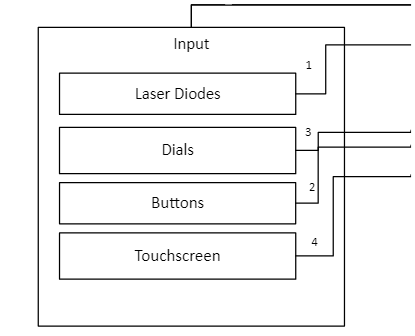
\includegraphics[width=0.60\textwidth]{images/InputSubsystem.png}
 \caption{Input Layer subsystems}
\end{figure}

\subsection{Input Subsystems}
The hardware involved in these subsystems are laser diodes and photo-transistors which read the interruptions of the laser diodes. The dial is a physical knob that is a potentiometer to control as a volume input for an onboard speaker.  Two buttons are working in a circular list to change the octaves of the harp sounds. One button is used as a way to change the instrument which also works as a circular list. 

\subsection{Input Operating System}
The operating system for this layer is driven by a Raspberry Pi operating system which handles all the inputs and outputs of each subsystem.

\subsection{Layer Software Dependencies}
A description of any software dependencies (libraries, frameworks, etc) required by the layer.

\begin{figure}[h!]
	\centering
 	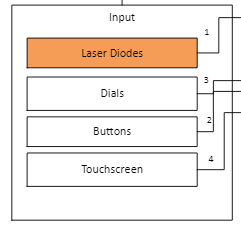
\includegraphics[width=0.60\textwidth]{images/Laserdiodes.png}
 \caption{Laser Diode Subsystem}
\end{figure}

\subsection{Laser Diodes}
This layer handles the input of the playing the harp as it is the harp's strings. The laser shines into the phototransistor at all times, when a finger blocks the laser the corresponding note is played. 


\subsubsection{Laser Diodes}
The laser diodes and phototransistors make up the hardware for the subsystem.

\subsubsection{Subsystem Operating System}
A description of any operating systems required by the subsystem.

\subsubsection{Subsystem Data Structures}
A description of any classes or other data structures that are worth discussing for the subsystem. For example, data being transmitted from a microcontroller to a PC via USB should be first be assembled into packets. What is the structure of the packets?

\subsubsection{Subsystem Data Processing}
A description of any algorithms or processing strategies that are worth discussing for the subsystem. If you are implementing a well-known algorithm, list it. If it is something unique to this project, discuss it in greater detail.


\begin{figure}[h!]
	\centering
 	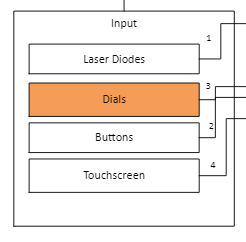
\includegraphics[width=0.60\textwidth]{images/Dials.png}
 \caption{Volume Control}
\end{figure}
\subsection{Volume Control}
This layer handles the input of a potentiometer to act as a volume control in conjunction with the GUI.


\subsubsection{Volume Control}
A single potentiometer will make up the hardware for this subsystem.

\subsubsection{Subsystem Operating System}
A description of any operating systems required by the subsystem.

\subsubsection{Subsystem Data Structures}
A description of any classes or other data structures that are worth discussing for the subsystem. For example, data being transmitted from a microcontroller to a PC via USB should be first be assembled into packets. What is the structure of the packets?

\subsubsection{Subsystem Data Processing}
A description of any algorithms or processing strategies that are worth discussing for the subsystem. If you are implementing a well-known algorithm, list it. If it is something unique to this project, discuss it in greater detail.
